\section{Redes de Hopfield}

\begin{frame}{Redes de Hopfield}%
  \justifying%
  Uma rede de Hopfield é uma rede que armazena padrões de tal forma que quando um padrão novo é mostrado para a rede, ela responde devolvendo o padrão que tem armazenado mais próximo ao novo padrão.
  \\~\\
  Hopfield é uma rede determinística.
\end{frame}

\subsection{Definições}
\begin{frame}{Quais os elementos básicos para Hopfield?}%
  \justifying%
  Vamos considerar que cada uma das \textbf{unidades} da rede é denominada por $\mathrm{x}_{i}$, onde $i = 1, \dots, N$, para uma rede com $N$ unidades.
  \\~\\
  Em Hopfield, cada $\mathrm{x}_{i}$ pode assumir um dos valores $x_{i} \in \{0, 1\}$. Rede binária!
  \\~\\
  Se $x_{i} = 0$, a unidade $i$ desativada; se $x_{i} = 1$, unidade $i$ ativada.
\end{frame}

\begin{frame}{Quais os elementos básicos para Hopfield?}%
  \justifying%
  Os \textbf{pesos} chamaremos de $\omega$.
  \\~\\
  Na rede de Hopfield os pesos são simétricos, isto é, $\omega_{ij} = \omega_{ji}$ (conexão entre as unidades $i$ e $j$).
\end{frame}

\subsection{Esquema}
\begin{frame}{Rede de Hopfield diagrama}
  \begin{figure}[h]{}%
    \label{fig:hopfield}%
    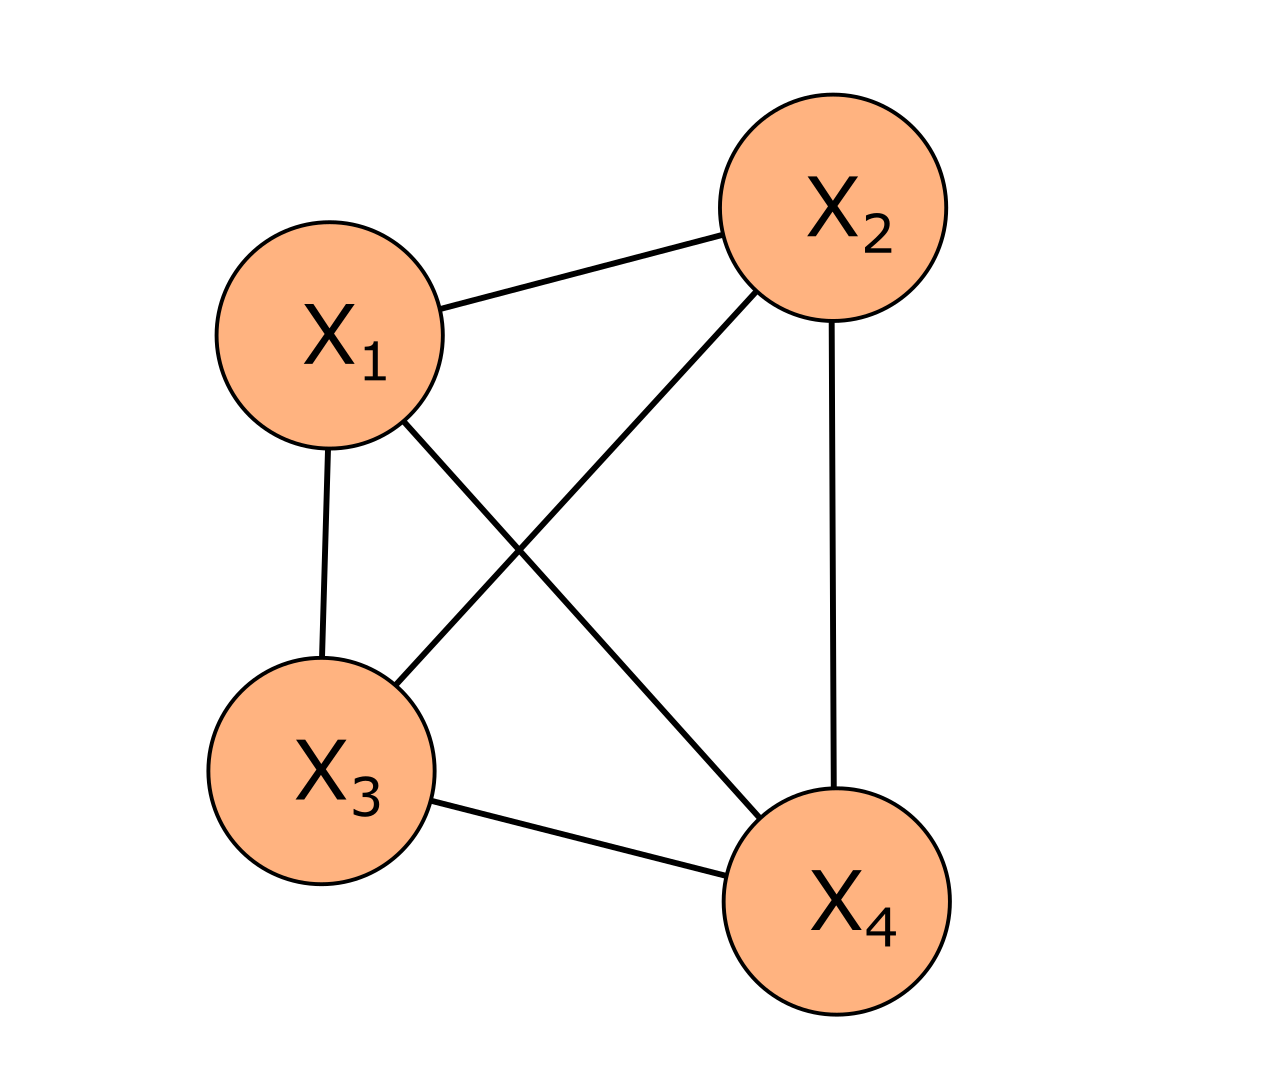
\includegraphics[scale=0.5]{images/hopfield.png}
    \caption{Distribuição dos neurônios de uma rede de Hopfield com 4 unidades.}
  \end{figure}
\end{frame}

\begin{frame}{Rede de Hopfield diagrama}
  \begin{figure}[h]{}%
    \label{fig:hopfield-full}%
    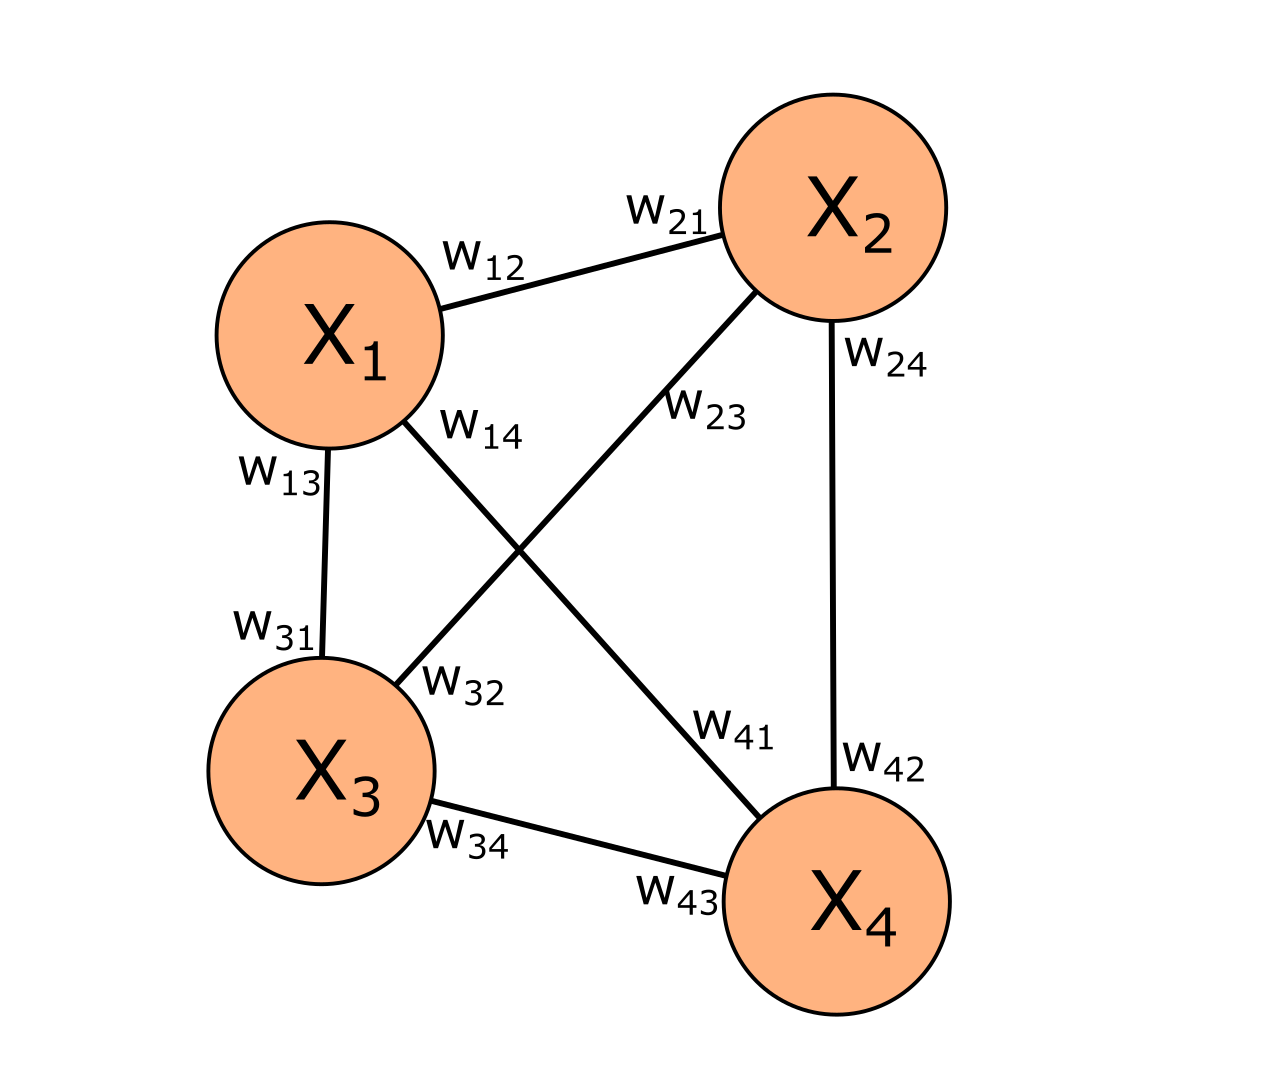
\includegraphics[scale=0.5]{images/hopfield_full.png}
    \caption{Identificação das conexões de uma rede de Hopfield com 4 unidades.}
  \end{figure}
\end{frame}

\begin{frame}{Estado da Rede}%
  \justifying%
  \onslide<1->{%
  Exemplo de um estado $\mathrm{\mathbf{x}}$ para uma rede binária com 4 unidades:}
  \onslide<2->{%
  \begin{align}%
    \label{eq:net-state}%
    \mathbf{x} &= (x_{1}, x_{2}, x_{3}, x_{4}) \nonumber \\
               &= (0, 1, 1, 0) \nonumber
  \end{align}
  }
\end{frame}

\subsection{Funcionamento}
\begin{frame}{Função de Energia}%
  \justifying%
  Segundo \textbf{HOPFIELD (1982)}, como as conexões são simétricas, existe uma função de energia $H$ para a rede, dado o estado $\mathrm{\mathbf{x}}$ em que ela se encontra.
  \begin{equation}%
    \label{eq:hopfield-energy-function}%
    H(\mathbf{x}) = - \frac{1}{2} \sum_{i} \sum_{j} \omega_{ij} x_{i} x_{j} - \sum_{i} \phi_{i} x_{i},
  \end{equation}
  \\~\\
  Equação~(\ref{eq:hopfield-energy-function}) depende da correlação entre as unidades (primeiro termo), e depende do limiar de ativação de cada unidade (segundo termo). Por simplificação podemos considerar apenas o primeiro termo.
  \\~\\
%  A energia sempre decresce ou permanece constante conforme o sistema evolui.
%  Sistema é estacionário quando a energia é menor. Achou um mínimo.
\end{frame}

\begin{frame}{Aprendizagem}%
  \justifying%
  Fazer a rede de Hopfield aprender corresponde a determinar os valores das conexões $\omega_{ij}$, a partir de um conjuto de padrões apresentado para a rede. Isto é, aprender quais são os mínimos da rede para o conjunto de treinamento em questão,
  \begin{equation}%
    \label{eq:hop-omega}
    \omega_{ij} = \frac{1}{N} x_{i} x_{j}.
  \end{equation}
  (considerando que a rede aprende apenas um padrão.)
\end{frame}

\begin{frame}{Função de Ativação}%
  \justifying%
  O valor $x_{i}$ que a unidade $\mathrm{x}_{i}$ possui é dada pela função degrau.
  \begin{figure}[h]{}%
    \label{fig:hopfield-step}%
    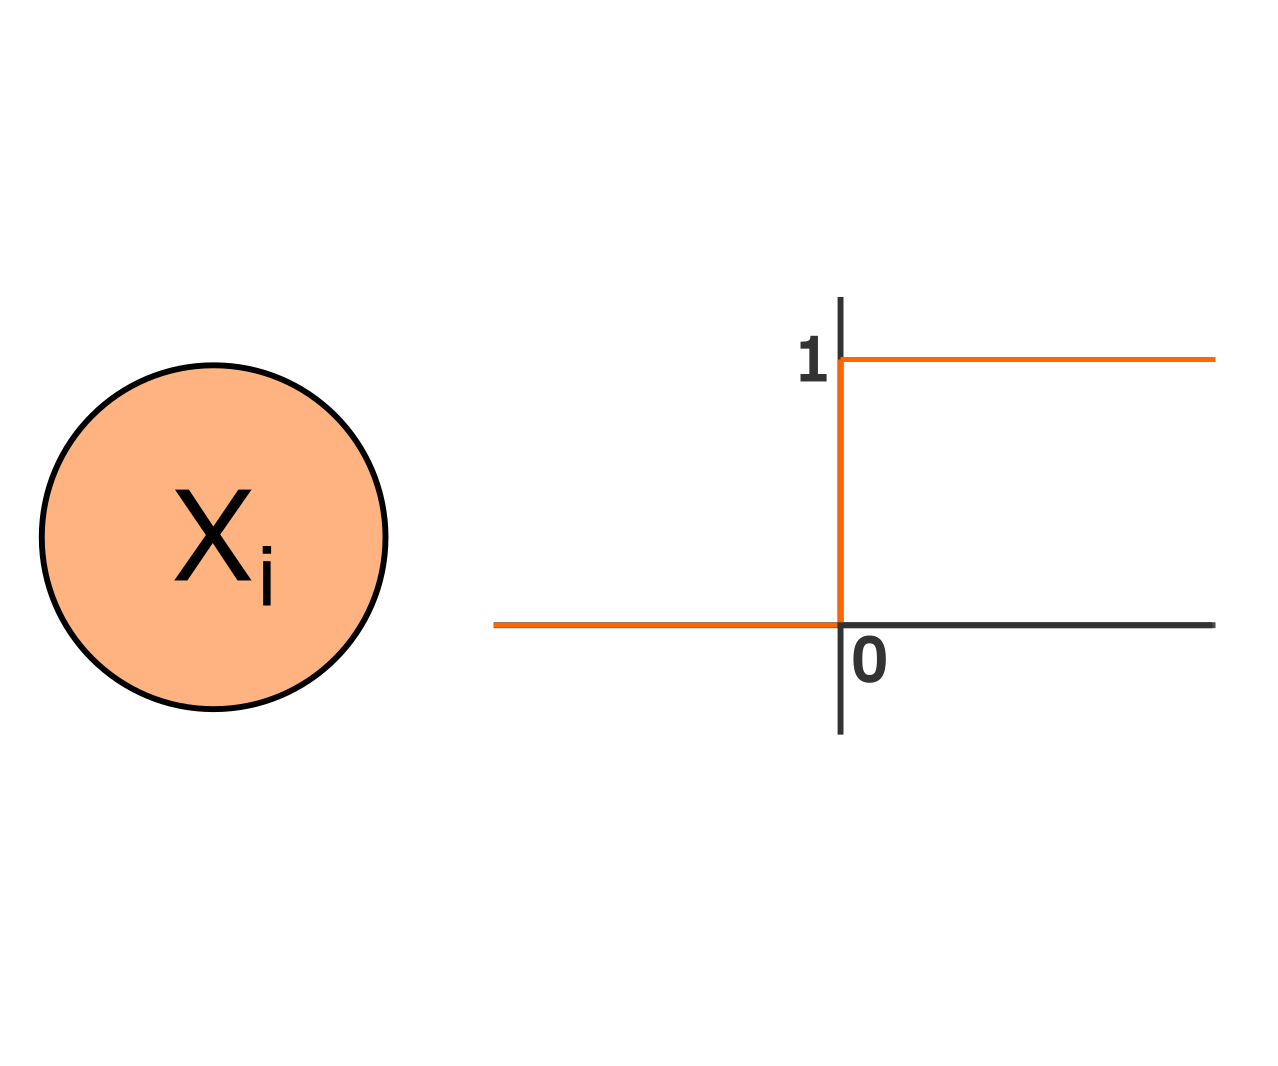
\includegraphics[scale=0.35]{images/hopfield_activation.png}
    \caption{Função de ativação de uma unidade na rede de Hopfield.}
  \end{figure}
  \begin{equation}%
    \label{eq:step-function}
    x_{i} = \Theta \left(\sum_{j} \omega_{ij} x_{j} \right)
  \end{equation}
\end{frame}

\begin{frame}{Funcionamento da rede de Hopfield}%
  \justifying%
  Uma vez que a rede determinou o valor de suas conexões, podemos mostrar um novo estado para a rede, por exemplo, $\mathrm{\mathbf{x}} = (1, 1, 0, 0)$.
  \\~\\
  Partindo de uma unidade escolhida aleatoriamente, determinamos se a unidade fica ativa ou não (muda de valor) avaliando a diferença de energia 
  \begin{equation}%
    \label{eq:energy-delta}%
    \Delta H_{i} = H_{i}(x_{i} = 0) - H_{i}(x_{i} = 1). 
  \end{equation}

\end{frame}

\begin{frame}{Funcionamento da rede de Hopfield}%
  Hopfield tem característica determinista porque a rede sempre opera indo em direção a menor energia.
  \\~\\
  Pode acontecer de ficar preso em mínimo local.
  \\~\\
  Em um problema com muitas variáveis, isso pode ser tornar um problema, pois podemos não chegar ao melhor resultado. Há outras formas de se contornar isso!
\end{frame}
